\documentclass[sigconf]{acmart}

\settopmatter{printacmref=false}
\renewcommand\footnotetextcopyrightpermission[1]{}
\pagestyle{plain}

\usepackage{graphicx}
\usepackage{booktabs}
\usepackage{multirow}
\usepackage{enumitem}
\usepackage{array}
\usepackage{hyperref}

\acmConference
[Human-Computer Interaction]
{Term Project: Human-Centered AI System (Final Report)}
{2026}
{IUT, OIC, Dhaka, Bangladesh}

\title{Explaining Before Installing: An Explainable AI Privacy Risk
Report that Improves User Comprehension of Android Application Behaviour}

%% ---------------------------------------------------------------
%% TODO: replace the three student author blocks with real names,
%% student IDs and institutional e-mail addresses before submission.
%% ---------------------------------------------------------------
\author{Author One}
\affiliation{
  \institution{Department of Computer Science and Engineering\\
  Islamic University of Technology (IUT), OIC}
  \city{Dhaka}
  \country{Bangladesh}
}
\email{author1@iut-dhaka.edu}

\author{Author Two}
\affiliation{
  \institution{Department of Computer Science and Engineering\\
  Islamic University of Technology (IUT), OIC}
  \city{Dhaka}
  \country{Bangladesh}
}
\email{author2@iut-dhaka.edu}

\author{Author Three}
\affiliation{
  \institution{Department of Computer Science and Engineering\\
  Islamic University of Technology (IUT), OIC}
  \city{Dhaka}
  \country{Bangladesh}
}
\email{author3@iut-dhaka.edu}

\author{Hasan Mahmud}
\affiliation{
  \institution{SSL, Department of Computer Science and Engineering\\
  Islamic University of Technology (IUT), OIC}
  \city{Dhaka}
  \country{Bangladesh}
}
\email{hasan@iut-dhaka.edu}
\authornote{Corresponding author.}

\begin{document}

\begin{abstract}
Application stores disclose what data an application collects, but they do
not tell a user whether that collection is reasonable. The Android
\emph{Data safety} section, for example, lists categories such as
``Personal info'' and ``Device or other IDs'' without conveying how much
privacy risk the combination represents or why. Users are therefore given
transparency without interpretability. We present an explainable
AI (XAI) based privacy risk assessment and decision support system that
converts static application features into a graded privacy risk score, uses
SHAP to identify the features responsible for that score, and renders those
factors as a short, plain-language justification shown before installation.
We evaluated the resulting interface against the current Google Play
\emph{Data safety} page in a within-subjects study with 34 participants.
Comprehension of the privacy risk rose from $M=2.15$ to $M=3.79$ on a
five-point scale (Wilcoxon signed-rank, $p<.001$, $r_{rb}=0.80$), and the
ability to understand the information without technical knowledge rose from
$M=2.18$ to $M=3.85$ ($p<.001$, $r_{rb}=0.82$). In forced choice, 31 of 34
participants preferred the explanatory interface on every comparative item
($p<.001$). The contribution of this work is not a new malware detector but
the demonstration that an explanation layer placed between a risk model and
an end user measurably changes what non-expert users understand about an
application before they install it, together with design guidance on how
brief such explanations must be to remain useful.
\end{abstract}

\keywords{Human-Centered AI, Interaction Design, Usability, Explainable AI,
HCI, Android Privacy, Decision Support}

\maketitle

% ====================================================
\section{Introduction}

Mobile applications routinely request access to contacts, precise location,
messages, device identifiers and network services. Both major application
stores now require developers to declare these practices, and Android
surfaces them in a \emph{Data safety} section on every store listing. The
disclosure problem is, in a narrow sense, solved: the information is
present, standardised and easy to find.

The interpretation problem is not. A user reading that an application
collects ``Personal info,'' ``Device or other IDs,'' ``App activity'' and
``Location'' receives four category labels and no basis on which to judge
them. The labels do not say whether this combination is ordinary for the
type of application being installed, which of the declared behaviours
matters most, or what the practical consequence of the combination might
be. Felt et al.~\cite{felt2012permissions} showed more than a decade ago
that only a small minority of users both notice and correctly interpret
Android permission information, and later work on privacy labels reports
that structured disclosures still fail to answer the questions users
actually have~\cite{zhang2022datasafety}. Disclosure has improved;
comprehension has not followed.

Two lines of work address parts of this gap without closing it. Privacy
nutrition labels~\cite{kelley2009nutrition} and personalised privacy
assistants~\cite{liu2016privacyassistant} make privacy information more
legible and more actionable, but they still present \emph{what} is
collected rather than \emph{how concerning} it is. Machine learning work on
Android security~\cite{arp2014drebin, wang2014permissionrisk,
yerima2019droidfusion} produces accurate risk and malware classifiers, but
their output is a label or a probability aimed at analysts, and a user told
only that an application scores $0.84$ is no better placed to decide than
one reading a category list. Neither tradition supplies the missing piece: a
justification, in ordinary language, of why this particular application is
being flagged.

We therefore treat the problem as one of human-centred AI rather than of
classification accuracy. Our system assesses privacy risk from static
application features, attributes that assessment to specific features using
SHAP~\cite{lundberg2017shap}, and translates the attributed features into a
two-to-three sentence justification presented alongside a graded risk score
at the moment of the install decision. The risk judgement remains with the
model; the language layer is constrained to restate what the model and the
attribution actually found, never to reach an independent verdict. The user
remains the decision maker, and the interface is explicit that an automated
assessment indicates potential concern rather than proven misuse.

This paper makes three contributions.

\begin{enumerate}[leftmargin=*, itemsep=2pt]
  \item \textbf{An explanation architecture for privacy risk.} We describe a
  pipeline---feature extraction, gradient-boosted risk assessment, SHAP
  attribution, constrained natural-language generation, decision-support
  interface---in which every user-visible sentence is traceable to a model
  attribution rather than generated freely.
  \item \textbf{Empirical evidence that the explanation layer changes
  comprehension.} In a within-subjects study with 34 participants, the
  explanatory interface produced large, statistically significant
  improvements in both understanding of the risk and understanding without
  technical background, relative to the deployed Google Play
  \emph{Data safety} page.
  \item \textbf{Design implications for explanation length and form.}
  Participant feedback converged on a constraint that the quantitative
  results alone would have hidden: the explanation must be short and
  scannable. Prose that is more complete but longer was explicitly rejected
  (``I don't want to read a novel''), which sharpens existing XAI guidance
  for consumer-facing, pre-decision contexts.
\end{enumerate}

% ====================================================
\section{Related Work}

\subsection{Communicating Mobile Privacy to Non-Experts}

Research on Android permissions has consistently found a comprehension
rather than an exposure problem. Felt et al.~\cite{felt2012permissions}
reported that most users neither attended to nor understood install-time
permission requests. Lin et al.~\cite{lin2012expectation} showed that user
concern depends less on which permission is requested than on whether the
request matches the expected purpose of the application---a location
request from a maps application and the same request from a flashlight
application are judged very differently. This finding motivates a central
design decision in our work: the explanation is written in terms of what
the combination of behaviours enables, not as an enumeration of permission
strings.

Structured disclosure formats improve legibility. The privacy nutrition
label~\cite{kelley2009nutrition} demonstrated that a standardised layout
speeds accurate information retrieval, and Kelley et
al.~\cite{kelley2013privacy} showed that privacy information placed in the
application selection flow shifts choices. Nudging studies report similar
effects in the field~\cite{almuhimedi2015nudges}. However, evaluations of
the deployed Data safety labels find that they still do not answer users'
actual questions~\cite{zhang2022datasafety}. All of these formats share a
structural property: they report \emph{what} is collected. Our system adds
an assessment of \emph{how concerning} the collection is, and a reason for
that assessment.

\subsection{Explainable AI and Its Human Evaluation}

Feature-attribution methods such as LIME~\cite{ribeiro2016lime} and
SHAP~\cite{lundberg2017shap, lundberg2020treeshap} identify the inputs
responsible for a prediction, and are the standard choice for tree
ensembles. Their limitation for our purpose is that their native output---a
ranked list of feature names with signed contributions---is a technical
artefact. Lipton~\cite{lipton2018mythos} and Doshi-Velez and
Kim~\cite{doshivelez2017rigorous} argue that interpretability claims must
be evaluated against a stated purpose and audience rather than asserted,
and Miller~\cite{miller2019explanation} draws on social science to show
that human explanation is selective and contrastive rather than exhaustive.
Kaur et al.~\cite{kaur2020interpreting} found that even data scientists
over-trust attribution tools they do not fully understand, and Bansal et
al.~\cite{bansal2021wholeexceeds} report that explanations can increase
acceptance of AI output without improving decision quality.

These results shape both our design and our claims. We do not present raw
SHAP values to users; we use them as the content constraint for a short
justification. We also deliberately restrict our claim to comprehension and
preference, which our study measured, rather than to decision correctness,
which it did not.

\subsection{Human-Centered AI Principles}

Shneiderman's framework~\cite{shneiderman2022hcai, shneiderman2020bridging}
argues for systems that are simultaneously highly automated and highly
controllable, and the Guidelines for Human-AI
Interaction~\cite{amershi2019guidelines} specify concrete obligations:
make clear what the system can do, make clear how well it does it, and
support efficient correction. Liao et al.~\cite{liao2020questioning} derive
an XAI question bank from practitioner interviews, in which ``why this
outcome'' and ``what would change it'' dominate. Interaction design
texts~\cite{sharp2019interaction} and goal-directed
design~\cite{cooper2014aboutface} supply the complementary requirement that
the artefact be organised around a user goal---here, deciding whether to
install---rather than around the structure of the underlying computation.

\subsection{Research Gap}

Existing work either makes privacy disclosures more legible without
assessing them, or assesses application risk accurately without explaining
the assessment to a non-expert. The gap we address is the junction: an
assessment that is attributed, translated into ordinary language, bounded
in its claims, and placed at the point of decision---and, critically, an
empirical test of whether that junction changes what ordinary users
understand.

% ====================================================
\section{Method (Integrating Assignment 1 and 2)}

This section integrates the requirements analysis of Assignment 1 with the
design and prototyping work of Assignment 2, and shows how the evidence
gathered about users determined the form of the final interface.

\subsection{Requirement Analysis (Assignment 1)}

\subsubsection{Users and Stakeholders}
The primary users are ordinary Android users who install applications from
an application store and have no security or machine-learning background.
Secondary stakeholders include application store operators, who bear the
consequence of misleading risk communication, and application developers,
whose products may be penalised by an unclear or unjustified warning. The
distinction matters for design: a system that labels applications without
justification transfers reputational risk to developers without giving
users a basis to evaluate the label.

\subsubsection{Data Gathering}
We used a structured questionnaire administered online, supplemented by
inspection of the deployed Google Play \emph{Data safety} page as an
artefact analysis. A questionnaire was chosen over interviews because the
research question concerns comparative comprehension across a population
of non-expert users rather than the depth of any individual's mental model,
and because a between-interface comparison requires a consistent stimulus
for every respondent. The artefact analysis established the baseline
condition and fixed the vocabulary---``Data shared \& collected'',
``Personal info'', ``Device or other IDs''---that the proposed interface
would have to improve upon.

\subsubsection{Analysis Method}
Closed items were analysed descriptively and comparatively. Free-text
responses were analysed with thematic analysis following Braun and
Clarke~\cite{braun2006thematic}: responses were coded independently, codes
were grouped into candidate themes, and themes were reviewed against the
full response set. With a small free-text corpus this yields orientation
rather than saturation, and we treat the themes accordingly.

\subsubsection{Personas and Scenarios}

\textbf{Persona 1 --- Rifat, 22, undergraduate student.} Installs
applications several times a month, mostly on recommendation. Scrolls past
the Data safety section because the categories mean nothing to him
concretely. Goal: avoid installing something that will quietly harvest his
contacts, without having to become an expert. Frustration: every
application appears to collect everything, so the disclosure gives him no
way to discriminate.

\textbf{Persona 2 --- Nusrat, 27, working professional.} Privacy-conscious
and moderately technical. Reads the permission list and can name what each
permission does, but cannot judge whether a given \emph{combination} is
excessive for the application's stated purpose. Goal: a defensible reason
to accept or reject an application in under a minute.

\textbf{Scenario.} Rifat finds a note-taking application and a messaging
application. Both declare access to device information and messaging
functions. The store presents both disclosures in the same neutral format.
He needs to know that in one case the combination is routine and in the
other it is not, and he needs that distinction before, not after,
installation.

\subsubsection{Task Analysis}
The pre-install privacy decision decomposes into four steps: (1) locate
privacy information on the store listing; (2) interpret the declared
behaviours; (3) judge whether those behaviours are proportionate to the
application's purpose; (4) decide to install or seek an alternative. The
deployed interface supports step~1 well and steps~2--3 poorly. Our design
targets steps~2 and~3 specifically, and leaves step~4 to the user.

\subsubsection{Requirements}

\textbf{Functional requirements.}
\begin{itemize}[leftmargin=*, itemsep=1pt]
  \item[FR1] Produce a graded privacy risk level (Low / Medium / High) with
  a bounded numeric score for an application.
  \item[FR2] Identify the application features that contributed most to
  that assessment.
  \item[FR3] Present those contributing factors as a short, non-technical
  justification.
  \item[FR4] State explicitly that the assessment is automated and
  indicative, not a determination of malicious behaviour.
  \item[FR5] Provide access to the underlying detailed application
  information for users who want it.
  \item[FR6] Present the assessment before the install decision is taken.
\end{itemize}

\textbf{Non-functional requirements.}
\begin{itemize}[leftmargin=*, itemsep=1pt]
  \item[NFR1] The justification must be comprehensible without security or
  machine-learning knowledge.
  \item[NFR2] The assessment must be readable within a short glance,
  consistent with store browsing behaviour.
  \item[NFR3] Visual risk encoding must be consistent and
  non-alarmist.
  \item[NFR4] Every user-visible claim must be traceable to a model
  attribution.
\end{itemize}

\subsubsection{Requirements--Goal Traceability}
Table~\ref{tab:trace} maps each requirement to the user goal that motivates
it and to the interface element that satisfies it.

\begin{table}[t]
\caption{Requirements--goal traceability matrix.}
\label{tab:trace}
\small
\begin{tabular}{@{}p{0.06\columnwidth}p{0.36\columnwidth}p{0.42\columnwidth}@{}}
\toprule
\textbf{Req} & \textbf{User goal} & \textbf{Interface element} \\
\midrule
FR1 & Judge severity at a glance & Risk badge, score /100, gauge bar \\
FR2 & Know what drove the judgement & Content of ``Why this assessment?'' \\
FR3 & Understand without expertise & Plain-language justification text \\
FR4 & Avoid over-trusting the system & ``Important note'' disclaimer block \\
FR5 & Verify independently & ``Review app information'' link \\
FR6 & Decide before committing & Placement on the pre-install screen \\
NFR1 & Understand without expertise & No permission strings in body text \\
NFR2 & Decide quickly & Single screen, no scrolling to reach verdict \\
NFR3 & Calibrate concern & Green/amber/red used only on the risk band \\
NFR4 & Trust the reason given & Generation constrained to SHAP output \\
\bottomrule
\end{tabular}
\end{table}

\subsection{Design and Prototyping (Assignment 2)}

\subsubsection{Design Rationale}
Four decisions follow directly from the requirements above.

\emph{A graded score rather than a binary verdict.} Step~3 of the task
analysis is a proportionality judgement, which a binary safe/unsafe label
cannot support. A 0--100 score with three named bands (FR1) allows a user
to distinguish a routine application from a borderline one.

\emph{Explanation in terms of capability, not permission.} Lin et
al.~\cite{lin2012expectation} show that users reason about purpose, not
permission identifiers. The justification therefore refers to ``messaging
functions'' and ``device identification'' rather than \texttt{SEND\_SMS} or
\texttt{READ\_PHONE\_STATE}, satisfying NFR1.

\emph{An explicit epistemic boundary.} Given evidence that explanations can
inflate trust beyond warrant~\cite{bansal2021wholeexceeds}, every screen
carries a disclaimer that an automated assessment indicates potential risk
and does not prove misuse (FR4), in line with the Human-AI Interaction
guideline to make clear how well the system performs~\cite{amershi2019guidelines}.

\emph{Verdict above the fold, detail on demand.} NFR2 requires that the
risk level be readable without scrolling; FR5 requires that the underlying
detail remain reachable. The layout therefore places badge, score and gauge
at the top and defers full application information to a link.

\subsubsection{Interaction Flow}
The user opens an application listing, the assessment is computed and
displayed, the user reads the risk band and, if they wish, the
justification, optionally expands the detailed application information, and
then installs or abandons. The interface does not block installation at any
point; it informs it.

\subsubsection{Prototype}
Figure~\ref{fig:ifaceA} shows the baseline condition---the deployed Google
Play \emph{Data safety} page. Figure~\ref{fig:ifaceB} shows the proposed
interface across three risk bands.

\begin{figure}[t]
  \centering
  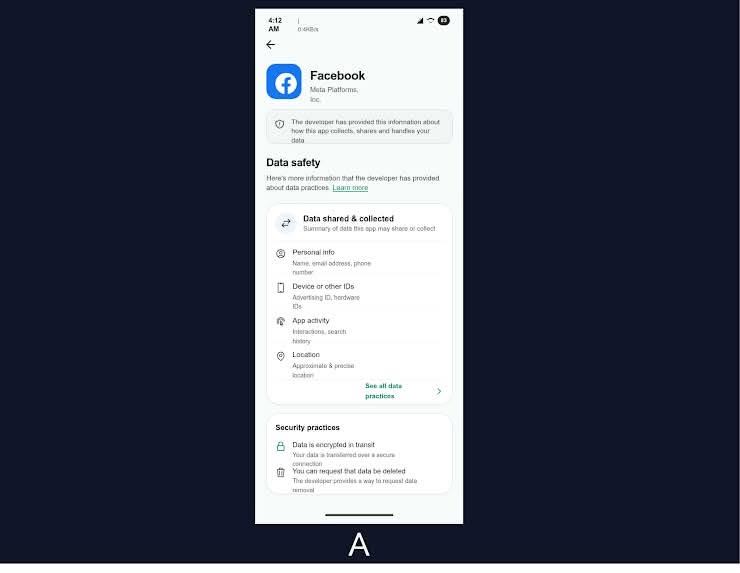
\includegraphics[width=0.72\columnwidth]{option-A_regular.jpg}
  \caption{Interface A (baseline): the deployed Google Play
  \emph{Data safety} page. Collection categories are disclosed; no
  assessment, ranking or justification is provided.}
  \label{fig:ifaceA}
\end{figure}

\begin{figure*}[t]
  \centering
  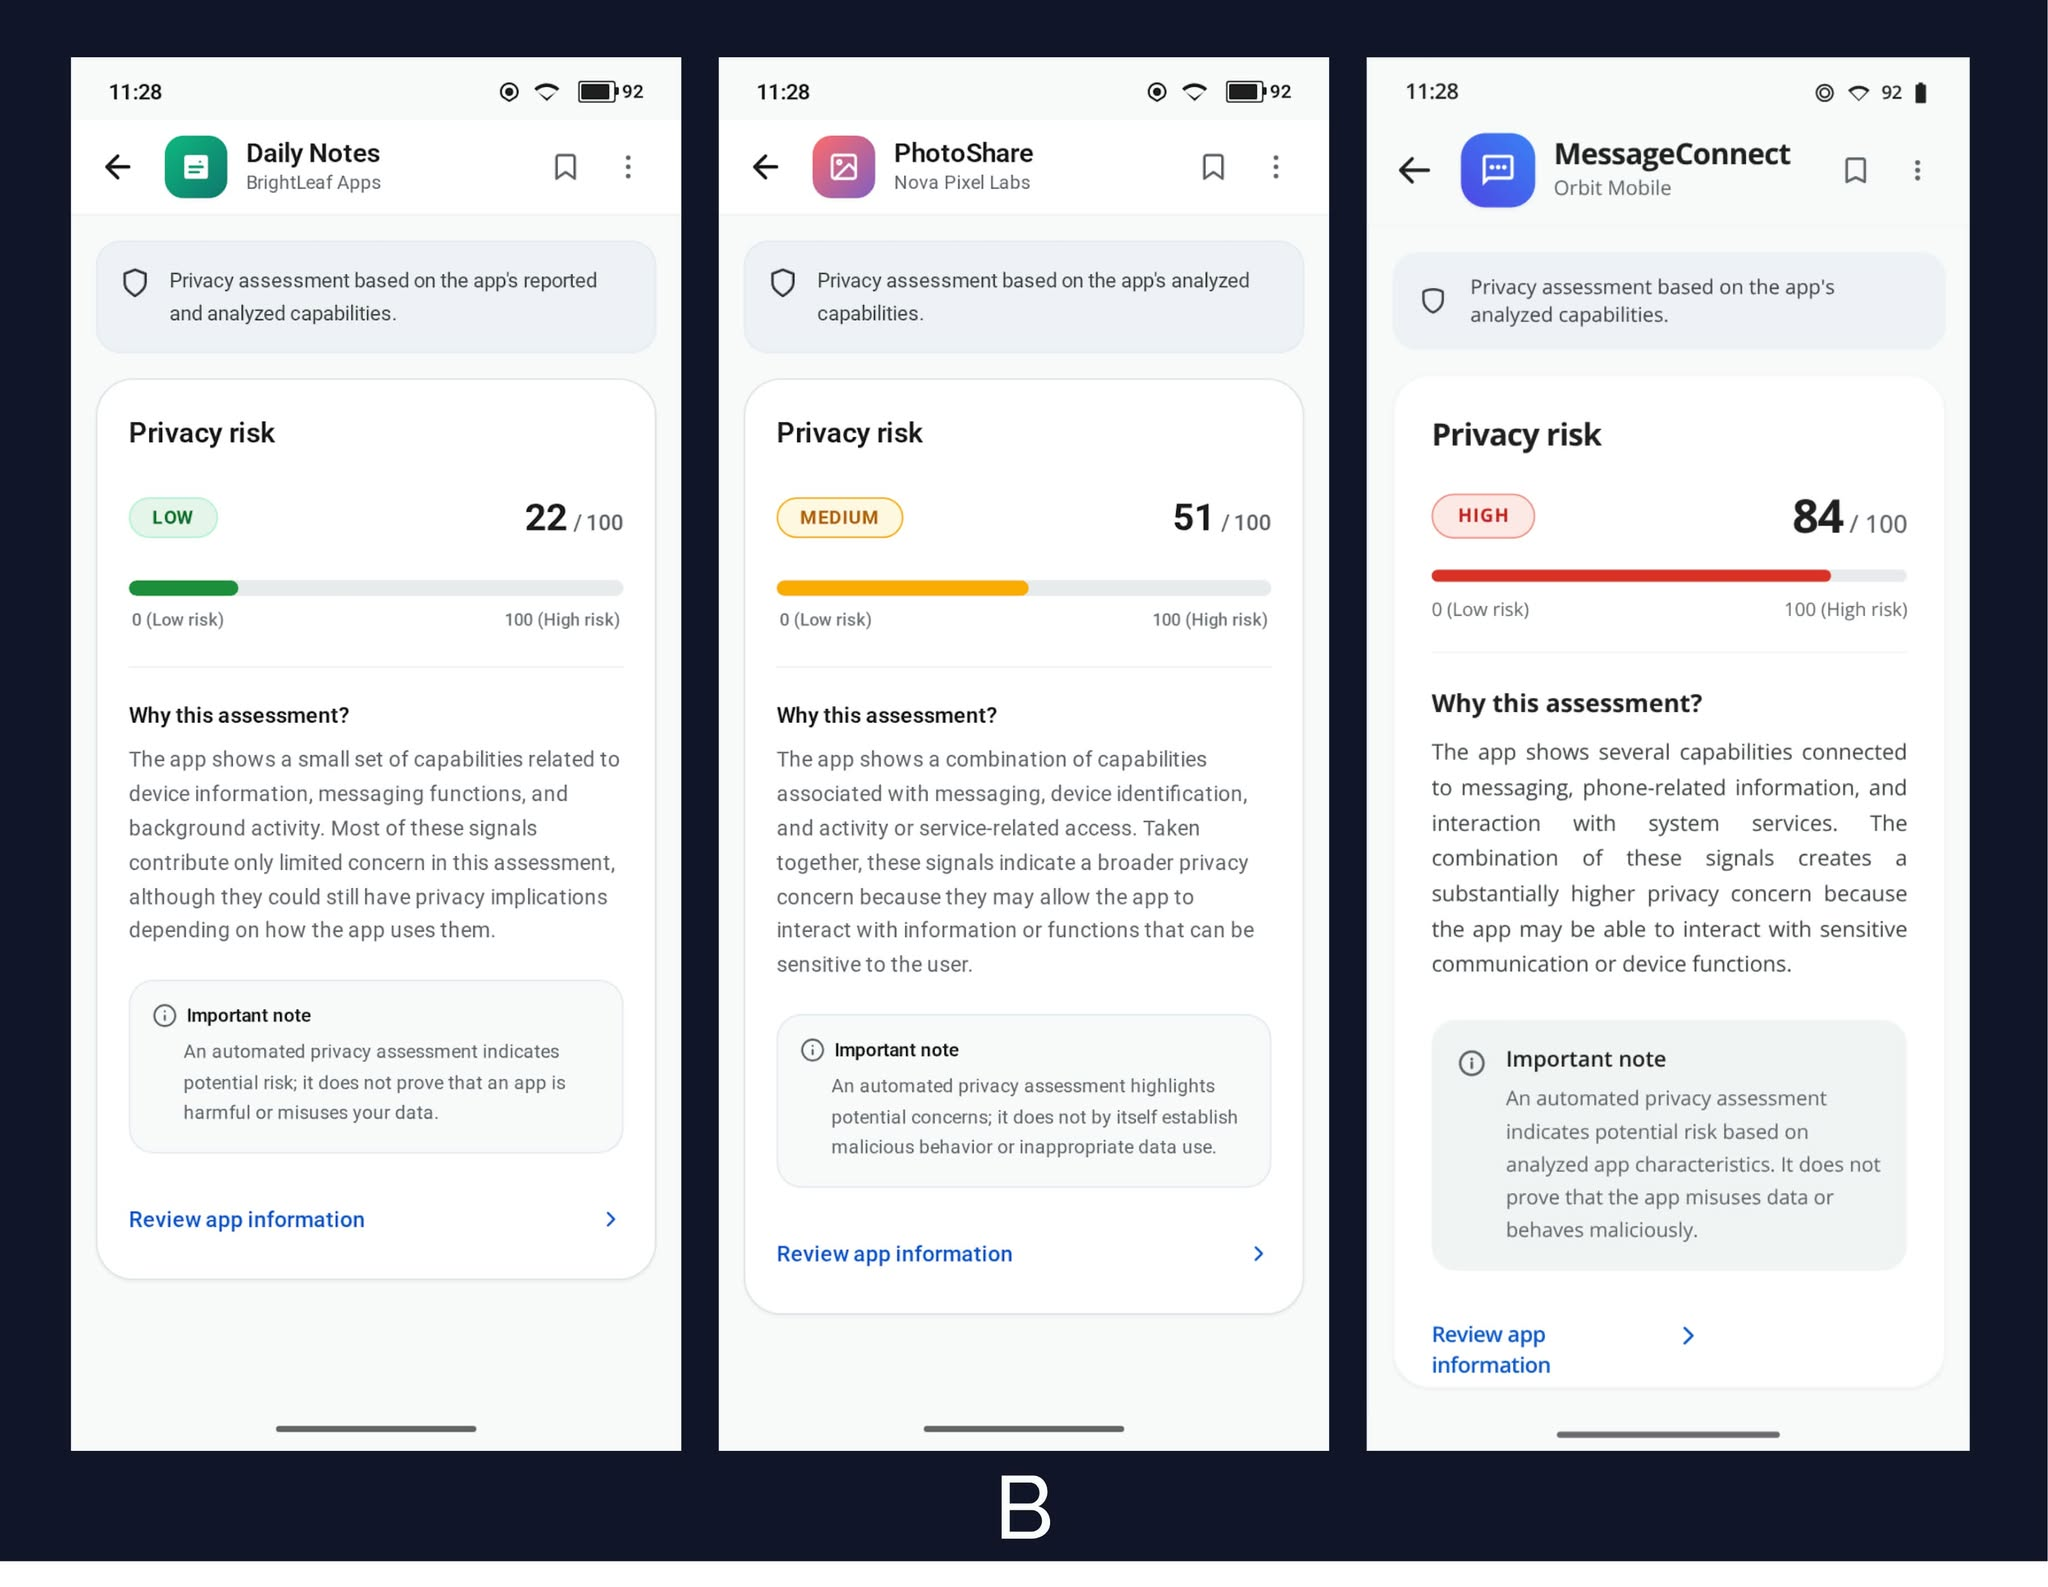
\includegraphics[width=0.92\textwidth]{OptionB_what_we_proposed.jpg}
  \caption{Interface B (proposed): the explainable privacy risk report at
  Low (22/100), Medium (51/100) and High (84/100) risk. Each screen pairs a
  graded score with a ``Why this assessment?'' justification derived from
  the model's feature attributions, an ``Important note'' stating the limits
  of an automated assessment, and a link to the detailed application
  information.}
  \label{fig:ifaceB}
\end{figure*}

\subsection{Human-Centered AI Considerations}

\textbf{Explainability.} The user is never shown a bare score. The ``Why
this assessment?'' block names the behavioural signals that produced the
score and states what their combination could enable, addressing the ``why
this outcome'' question that dominates practitioner XAI
needs~\cite{liao2020questioning}.

\textbf{Human control.} The system is advisory. It does not block, rank or
remove applications, and the install decision is never automated. The
``Review app information'' affordance lets a user inspect the evidence and
disagree with the assessment.

\textbf{Trust calibration.} Rather than maximising trust, the design bounds
it. The disclaimer is persistent and appears even on the Low-risk screen,
so that the limits of the assessment are communicated in the case where the
user has least incentive to read them.

% ====================================================
\section{System Design and Implementation}

\subsection{System Overview}

The system is a five-stage pipeline. An Android application package
supplies static features; a gradient-boosted classifier produces a privacy
risk assessment; SHAP attributes that assessment to individual features; a
constrained language layer converts the top-ranked attributions into a
short justification; and the decision-support interface presents score,
justification and disclaimer together before installation.

The separation between the training corpus and the runtime input is
deliberate. The model is trained on a labelled corpus of Android
application feature vectors, whereas at run time features are extracted
from an actual application package into the identical feature space. The
user is never shown the training data; they are shown an assessment of the
application in front of them.

\subsection{Functional Design and Features}

\textbf{Graded risk assessment (FR1).} The classifier output is mapped to a
0--100 score and to one of three bands. The gauge bar makes the position
within the band visible, so that a score of 51 does not read identically to
a score of 79.

\textbf{Factor identification (FR2).} SHAP values rank the features by
contribution to the individual prediction. Only the highest-contributing
features enter the explanation, consistent with the finding that human
explanation is selective rather than exhaustive~\cite{miller2019explanation}.

\textbf{Plain-language justification (FR3, NFR1, NFR4).} The language layer
receives the risk band and the ranked attributions and is constrained to
restate them. It does not have access to an independent judgement of the
application and cannot introduce a factor the model did not identify. This
constraint is what makes NFR4 checkable: every clause in the justification
corresponds to an attributed feature.

\textbf{Epistemic disclaimer (FR4).} Fixed text, not generated, so that it
cannot be weakened by the language layer.

\textbf{Detail on demand (FR5).} ``Review app information'' exposes the
underlying declared behaviours for users who want the primary evidence.

\subsection{Interface Design and Interaction Flow}

The screen is organised top to bottom in decreasing order of decision
value: application identity, scope statement, risk band and score,
justification, disclaimer, detail link. A user who reads only the first
third of the screen still obtains the verdict; a user who reads all of it
obtains the reason and its limits. Colour is applied only to the risk band
and gauge, so that the encoding remains unambiguous and the rest of the
screen stays neutral (NFR3).

\subsection{Human-Centered AI Implementation}

AI performs assessment and attribution only. It does not act, filter or
decide. Communication of the assessment is split across three registers---a
numeric score for magnitude, a colour band for immediate severity, and
prose for reasoning---so that a user who does not read the prose still
receives a calibrated signal. Override is implicit but total: the user
installs or does not.

\subsection{Implementation Details}

The risk model is a LightGBM gradient-boosting
classifier~\cite{ke2017lightgbm}, selected because the application
representation is high-dimensional, sparse and binary---conditions under
which gradient-boosted trees are strong and, equally important, under which
exact tree-based SHAP values are tractable~\cite{lundberg2020treeshap}.
Attribution uses the \texttt{shap} library's \texttt{TreeExplainer};
data handling and evaluation use scikit-learn~\cite{pedregosa2011scikit}.
The model is trained on a public corpus of static Android application
features, in which each application is represented as a binary vector over
requested permissions, declared intents and API-related behaviours.

\textbf{Implementation limitations.} The analysis is static. Behaviour that
appears only at run time, code loaded dynamically, and obfuscated or
packed payloads are outside its reach, and an application can therefore
present a benign static profile while behaving otherwise. The system is
positioned accordingly as a privacy risk indicator, not a malware
detector---a boundary the interface states to the user rather than leaving
implicit.

% ====================================================
\section{Evaluation}

\subsection{Experimental Design}

\textbf{Participants.} Thirty-four participants completed the study.
Table~\ref{tab:demo} reports the sample. The majority were aged 21--25
(79.4\%), with 11.8\% aged 18--20 and 8.8\% aged 26--30. Self-rated
familiarity with Android permissions and privacy information averaged
$M=3.29$ ($SD=1.02$) on a five-point scale, spanning the full range from 1
to 5, so the sample contains both low- and high-familiarity respondents
rather than only novices. Participants were recruited by convenience
sampling and were not compensated.

\begin{table}[t]
\caption{Participant demographics and self-reported background ($N=34$).}
\label{tab:demo}
\small
\begin{tabular}{@{}llr@{}}
\toprule
\textbf{Variable} & \textbf{Level} & \textbf{n (\%)} \\
\midrule
\multirow{3}{*}{Age group}
 & 18--20 & 4 (11.8) \\
 & 21--25 & 27 (79.4) \\
 & 26--30 & 3 (8.8) \\
\midrule
\multirow{4}{*}{Install frequency}
 & Rarely & 5 (14.7) \\
 & Occasionally & 13 (38.2) \\
 & Frequently & 11 (32.4) \\
 & Very frequently & 5 (14.7) \\
\midrule
\multirow{5}{*}{Permission familiarity}
 & 1 (none) & 1 (2.9) \\
 & 2 & 6 (17.6) \\
 & 3 & 14 (41.2) \\
 & 4 & 8 (23.5) \\
 & 5 (high) & 5 (14.7) \\
\bottomrule
\end{tabular}
\end{table}

\textbf{Design.} The study used a within-subjects design with interface as
the independent variable at two levels: Interface~A, the deployed Google
Play \emph{Data safety} page (Figure~\ref{fig:ifaceA}), and Interface~B,
the proposed explainable privacy report (Figure~\ref{fig:ifaceB}). A
within-subjects design was chosen because the dependent measures are
subjective comprehension ratings, which vary substantially between
individuals; having each participant rate both interfaces removes that
between-person variance and permits a direct paired comparison, which is
valuable at this sample size.

\textbf{Dependent variables.} Two five-point Likert items were collected
for each interface: ease of understanding the privacy risk presented, and
ease of understanding the information without technical knowledge. Three
forced-choice items then asked which interface made the risk easier to
understand, which explained the reason behind the risk more clearly, and
which the participant would prefer in practice. A free-text item asked for
the main improvement to the proposed interface.

\textbf{Context.} The evaluation was conducted remotely through an online
questionnaire, with both interfaces presented as static screen images. This
is a comprehension study of the presentation, not a usability study of a
live system; no interaction was logged.

\subsection{Procedure}

Participants first answered demographic and background questions. They were
then shown Interface~A, described as the privacy information currently
shown on an application store listing, and rated it on the two
comprehension items. They were then shown Interface~B across its three risk
bands, described as a proposed alternative, and rated it on the same two
items. The three forced-choice comparisons followed, with both interfaces
available for reference, and the questionnaire closed with the free-text
improvement item. No training was given, which is deliberate: the interface
is intended for users encountering it cold on a store listing, and any
briefing would have measured the briefing rather than the design.

\subsection{Evaluation Metrics}

Because the study evaluates comprehension of a static presentation rather
than performance on an interactive system, the conventional efficiency
measures---task completion time, error rate, number of interactions---do
not apply and were not collected. The measures used were:

\textbf{Quantitative.} (i) Perceived comprehension of the privacy risk;
(ii) perceived comprehension without technical knowledge; (iii) proportion
of participants selecting each interface on three forced-choice items.
Measures (i) and (ii) map directly to NFR1 and to steps~2--3 of the task
analysis, which is where the baseline was judged weakest. Measure (iii)
captures revealed preference, which is a stricter test than a rating
because it forces a comparison.

\textbf{Qualitative.} Free-text responses on the main improvement needed,
analysed thematically~\cite{braun2006thematic}.

\subsection{Analysis Approach}

Likert responses are ordinal and paired, so the two interfaces were
compared with the Wilcoxon signed-rank
test~\cite{wilcoxon1945individual} rather than a paired $t$-test. Effect
size is reported as the matched-pairs rank-biserial correlation $r_{rb}$,
on which $0.5$ is conventionally regarded as a large effect. Forced-choice
outcomes were tested against chance with a two-sided exact binomial test on
the participants expressing a preference, with ties excluded. The
significance threshold was $\alpha = .05$. Free-text responses were coded
and grouped into themes, which are reported with counts to keep their
weight visible given the small corpus.

% ====================================================
\section{Results}

\subsection{Quantitative Results}

Table~\ref{tab:likert} reports the paired comparison on both comprehension
measures. Interface~B was rated substantially higher on each.

\begin{table}[t]
\caption{Paired comparison of comprehension measures ($N=34$, five-point
scale). Wilcoxon signed-rank test; $r_{rb}$ is the matched-pairs
rank-biserial correlation.}
\label{tab:likert}
\small
\begin{tabular}{@{}lccc@{}}
\toprule
\textbf{Measure} & \textbf{A: $M$ ($SD$)} & \textbf{B: $M$ ($SD$)} & \textbf{Test} \\
\midrule
Understanding of & \multirow{2}{*}{2.15 (1.17)} & \multirow{2}{*}{3.79 (1.21)} & $p<.001$ \\
privacy risk & & & $r_{rb}=0.80$ \\
\addlinespace
Understanding without & \multirow{2}{*}{2.18 (1.10)} & \multirow{2}{*}{3.85 (1.06)} & $p<.001$ \\
technical knowledge & & & $r_{rb}=0.82$ \\
\bottomrule
\end{tabular}
\end{table}

Understanding of the privacy risk rose from $M=2.15$ ($SD=1.17$) for
Interface~A to $M=3.79$ ($SD=1.21$) for Interface~B, a difference of $1.64$
scale points ($W=40.0$, $p<.001$, $r_{rb}=0.80$, 26 non-tied pairs).
Understanding without technical knowledge rose from $M=2.18$ ($SD=1.10$) to
$M=3.85$ ($SD=1.06$), a difference of $1.67$ points ($W=32.5$, $p<.001$,
$r_{rb}=0.82$, 26 non-tied pairs). Both effects are large by conventional
interpretation.

The shape of the distributions is as informative as the means. For
Interface~A, 22 of 34 participants (64.7\%) gave a rating of 1 or 2 for
understanding the risk, and only 4 (11.8\%) gave 4 or 5. For Interface~B
the pattern inverts: 22 participants (64.7\%) gave 4 or 5, and 7 (20.6\%)
gave 1 or 2. The baseline was not merely rated lower on average; it failed
for a clear majority of the sample.

Table~\ref{tab:choice} reports the forced-choice items. On all three, 31 of
34 participants selected Interface~B, 2 selected Interface~A, and 1
recorded a tie or no preference. Among the 33 participants expressing a
preference, this is significant against chance on each item (two-sided
exact binomial, $p<.001$).

\begin{table}[t]
\caption{Forced-choice comparisons ($N=34$). Two-sided exact binomial test
on the 33 participants expressing a preference.}
\label{tab:choice}
\small
\begin{tabular}{@{}lcccc@{}}
\toprule
\textbf{Item} & \textbf{B} & \textbf{A} & \textbf{Tie} & \textbf{$p$} \\
\midrule
Easier to understand the risk & 31 & 2 & 1 & $<.001$ \\
Explained the reason more clearly & 31 & 2 & 1 & $<.001$ \\
Would prefer in practice & 31 & 2 & 1 & $<.001$ \\
\bottomrule
\end{tabular}
\end{table}

The three participants who did not prefer Interface~B on the overall
preference item are worth isolating rather than averaging away. One rated
Interface~A at the ceiling (5 on both measures) and Interface~B at the
floor, and supplied the free-text comment quoted below; this participant
also reported the highest install frequency and high familiarity. The
pattern is consistent with an experienced user for whom the baseline is
already sufficient and additional prose is overhead.

\subsection{Qualitative Findings}

Seven participants supplied free-text responses. Thematic analysis
produced three themes.

\textbf{Theme 1: Explanation length is a cost (2 responses).} The most
pointed response was ``I want to know what information they collect. I
don't want to read a novel.'' A second asked that the interface be made
``more convenient and easier or user friendly.'' Both locate the problem in
the volume of prose rather than its content.

\textbf{Theme 2: Structure over prose (1 response).} ``The assessment why
some app is risky could be written in bullet points to make it more clear
visually.'' This is a concrete alternative to the paragraph form: the same
attributed factors, rendered as a scannable list.

\textbf{Theme 3: Approval with a clarity reservation (4 responses).}
``It's all good''; ``UI is good. But should be more clear.''; ``UI'';
``N/A''. These endorse the direction while, in two cases, repeating that
clarity can improve.

No participant questioned the accuracy of the risk scores or asked how they
were computed---a silence we return to in the Discussion.

\subsection{Comparative Observations}

The two conditions differ in kind, not degree. Interface~A discloses
categories; Interface~B discloses categories, assesses them, ranks the
contributing factors and justifies the assessment. The comprehension gap of
roughly $1.65$ scale points, together with near-unanimous preference,
indicates that the addition is doing work. The near-identical results on
the two comprehension measures ($1.64$ and $1.67$ points; $r_{rb}=0.80$ and
$0.82$) suggest that for this sample, understanding the risk and
understanding it without technical background were not separable---the
baseline's failure was a single failure of interpretability, not two
distinct ones.

\subsection{Summary of Key Findings}

\textbf{What worked.} The graded score with a plain-language justification
produced large, significant gains on both comprehension measures and was
preferred by 91.2\% of participants on every comparative item.

\textbf{What did not.} The paragraph form of the justification was the one
consistently criticised element. Participants wanted the same information
in less space and in scannable structure.

\textbf{Unexpected.} No participant asked how the risk score was derived,
or expressed doubt about it, despite a persistent on-screen disclaimer
stating the assessment is automated and indicative. The explanation appears
to have satisfied curiosity about the verdict without prompting scrutiny of
the mechanism.

% ====================================================
\section{Discussion}

\subsection{Why the Explanatory Interface Won}

The baseline's weakness is not that it withholds information but that it
stops one step short of the user's actual task. Step~3 of our task
analysis---judging proportionality---requires a comparison between what an
application does and what its purpose warrants, and a category list
supplies only one side of that comparison. Interface~B supplies the other
side: it states which behaviours drove the assessment and what their
combination could enable. This is consistent with Lin et
al.~\cite{lin2012expectation}: users reason about purpose fit, and an
interface that speaks in those terms is doing less translation work for
them.

The equality of the two effect sizes supports this reading. If the
baseline's problem had been technical vocabulary alone, we would expect the
``without technical knowledge'' measure to improve more than the general
comprehension measure. They improved almost identically, which suggests the
missing element was interpretation itself rather than terminology---a gap
that better wording of a category list could not close.

\subsection{Which Design Decisions Held}

The graded score and colour band held: participants oriented to the verdict
without complaint, and no free-text response asked for a different risk
encoding. The disclaimer held in the weak sense that no participant
reported confusion about the system's authority, though as noted below its
effect on trust was not measured.

The paragraph justification did not hold. It satisfied the requirement to
explain (FR3) while violating the requirement to be readable at a glance
(NFR2), and participants detected the tension immediately. Our design
treated ``explanation'' and ``brevity'' as compatible; the data indicates
they trade off, and that in a pre-install context brevity has the stronger
claim. The bullet-point suggestion from Theme~2 is the natural resolution
and preserves the attribution chain, since the underlying SHAP ranking is
already a list---it was the rendering into prose that added the length.

\subsection{The Silence About the Model}

That no participant questioned how the score was computed is the finding we
regard with most caution. A benign reading is that the explanation answered
the question users had, making the mechanism irrelevant to them. A less
comfortable reading is that a fluent justification licensed acceptance of a
number without scrutiny---precisely the pattern Bansal et
al.~\cite{bansal2021wholeexceeds} report, where explanation increases
acceptance without improving decision quality, and Kaur et
al.~\cite{kaur2020interpreting} observe even among experts. Our study
cannot distinguish these, because it measured comprehension and preference
but not calibration: we never showed participants an incorrect assessment
to see whether they would catch it. Until that test is run, the
comprehension gain should not be read as evidence of appropriate trust.

\subsection{The Dissenting Participants}

The participant who preferred Interface~A rated their own familiarity at
the ceiling and installs applications very frequently. For such a user, the
category list is already interpretable and the justification is redundant
text between them and the decision. This suggests that explanation depth
should be responsive to user expertise rather than fixed---a progressive
disclosure design in which the verdict is always visible and the
justification expands on demand would serve both this participant and the
majority, and would simultaneously address the length complaint.

% ====================================================
\section{Implications for Design}

\textbf{1. For consumer pre-decision contexts, explanation length is a
usability constraint, not a presentation detail.} XAI guidance emphasises
selecting and contrasting~\cite{miller2019explanation}, but our
participants applied a harder budget: two to three sentences of prose were
already experienced as too much at the moment of an install decision.
Designers should treat the explanation's word count as a requirement with a
stated limit, tested like any other.

\textbf{2. Render attributions as structure, not prose.} Feature
attribution produces a ranked list. Converting it into paragraphs adds
reading time without adding information. Keeping the list form---short
labelled bullets in the user's vocabulary---preserves scannability and
shortens the distance between what the model computed and what the user
reads.

\textbf{3. Make explanation depth progressive.} A fixed explanation depth
cannot serve both a novice and an expert. Verdict always visible,
justification one tap away, evidence two taps away, satisfies both without
penalising either.

\textbf{4. Comprehension gains are not trust calibration, and should not be
reported as such.} Our study shows users understood the assessment better;
it does not show they would have rejected a wrong one. Any system in this
space should include at least one condition with a deliberately incorrect
assessment, or its evaluation cannot speak to over-reliance.

\textbf{5. State the epistemic boundary in fixed, non-generated text.} When
a language layer produces the explanation, the limits of the system should
not be within its reach to soften. Holding the disclaimer outside the
generated region is a small architectural decision with a direct effect on
what the system can be made to claim.

% ====================================================
\section{Limitations}

\textbf{Sample.} Thirty-four participants, recruited by convenience, of
whom 79.4\% were aged 21--25 and the majority of student background. The
sample is younger and more technically exposed than the Android user
population, and the results should not be generalised to older or less
digitally fluent users, who may need more explanation rather than less.

\textbf{Stimulus and measures.} Participants rated static images, not a
working system. All quantitative measures are self-reported perceived
comprehension; we did not test objective comprehension---for example by
asking participants to state what an application could do after reading
each interface. Perceived and actual understanding can diverge, and a
fluent explanation is exactly the condition under which they are most
likely to. Because the baseline used a real, recognisable application
(Facebook) while the proposed interface used fictional applications,
brand-related priors may have affected the baseline ratings; matching the
applications across conditions would remove this confound.

\textbf{Order effects.} All participants saw Interface~A before
Interface~B. Presentation order was not counterbalanced, so part of the
difference may reflect order or contrast rather than the design alone.

\textbf{Instrumentation.} Two of the four Likert items were mislabelled in
the deployed questionnaire, both referring to Interface~B where the first
of each pair concerned Interface~A. The intended mapping was confirmed and
the response distributions are internally consistent with it, but the
questionnaire text as administered was ambiguous and should be corrected
before reuse.

\textbf{Free-text corpus.} Seven responses support orientation, not
thematic saturation. The length theme is stated by two participants; its
prominence in our design implications reflects its specificity and its
convergence with the third theme's clarity reservations, not its frequency.

\textbf{System scope.} The analysis is static, and the risk model's
predictive performance is reported elsewhere in this paper as a design
property rather than validated against a held-out benchmark within this
study. The user evaluation tested the presentation of an assessment, not
the correctness of the assessment.

% ====================================================
\section{Conclusion}

We built an explainable AI privacy risk assessment and decision support
system for Android applications, which converts static application features
into a graded risk score, attributes that score to specific behavioural
features using SHAP, and presents the result as a short plain-language
justification at the point of the install decision. Evaluated against the
deployed Google Play \emph{Data safety} page with 34 participants, the
interface improved perceived comprehension of privacy risk by 1.64 points
on a five-point scale ($p<.001$, $r_{rb}=0.80$) and comprehension without
technical knowledge by 1.67 points ($p<.001$, $r_{rb}=0.82$), and was
preferred by 31 of 34 participants on every comparative item.

The contribution is the demonstration that an explanation layer between a
risk model and an end user changes what non-experts understand before they
install, together with the design constraint our participants imposed on
it: the explanation must be brief and scannable, or it becomes the new
obstacle. Attribution output should therefore reach the user as structure
rather than prose, and explanation depth should be progressive rather than
fixed.

Three directions follow. First, objective comprehension measures and a
deliberately incorrect-assessment condition, to determine whether the
comprehension gain corresponds to calibrated trust or to fluent
acceptance. Second, a counterbalanced study with matched applications
across conditions and a broader age range. Third, an interactive prototype
supporting progressive disclosure, which would allow the efficiency
measures---time to decision, depth of information sought---that a static
stimulus could not provide.

% ====================================================
\bibliographystyle{ACM-Reference-Format}
\bibliography{references}

\end{document}
